\section{Distribución Poisson}
\subsection{La Distribución de Poisson}
{Distribución de Poisson} Diremos que una variable aleatoria \emph{discreta} $X$ tiene distribución de Poisson si su función de probabilidad está dada por:
 \begin{align}
  \label{eq:2.10.7}
  f(n)=\dfrac{\lam^{n}e^{-\lam}}{n!}, \; n=0,1,2,...
 \end{align}


En este caso, $\mu_{X}=\s^{2}=\lam.$


\begin{quote}
 En teoría de probabilidad y estadística, la distribución de Poisson es una distribución de probabilidad discreta que expresa, a partir de una frecuencia de ocurrencia media, la probabilidad de que ocurra un determinado número de eventos durante cierto período de tiempo. Concretamente, se especializa en la probabilidad de ocurrencia de sucesos con probabilidades muy pequeñas, o sucesos raros.
\end{quote}

\href{https://es.wikipedia.org/wiki/Distribuci\%C3\%B3n_de_Poisson}{Wikipedia: Distribución de Poisson}


\begin{ejemplo}
  \label{exmp:2.10.5}
  El número de personas por día que llegan a una sala de urgencia tiene una distribución de Poisson con media 5. Hallar la probabilidad de que cuando mucho lleguen tres por día y la probabilidad de que por lo menos lleguen 8 personas por día.
 \end{ejemplo}

\begin{solucion}
	Usando la distribución de Poisson con $\lambda = 5$:

	\begin{enumerate}
		\item $P(X \leq 3) = \sum_{n=0}^{3} \frac{5^n e^{-5}}{n!}$
		\begin{align}
			&= \frac{5^0 e^{-5}}{0!} + \frac{5^1 e^{-5}}{1!} + \frac{5^2 e^{-5}}{2!} + \frac{5^3 e^{-5}}{3!} \\
			&= e^{-5}(1 + 5 + 12.5 + 20.833) \\
			&= e^{-5} \cdot 39.333 \approx 0.265
		\end{align}

		\item $P(X \geq 8) = 1 - P(X \leq 7)$
		\begin{align}
			&= 1 - \sum_{n=0}^{7} \frac{5^n e^{-5}}{n!} \\
			&\approx 1 - 0.867 = 0.133
		\end{align}
	\end{enumerate}
\end{solucion}




\lstinputlisting[language=Python]{../code/distribuciones-especiales/distPoisson.py}



 \begin{figure}
 \centering
 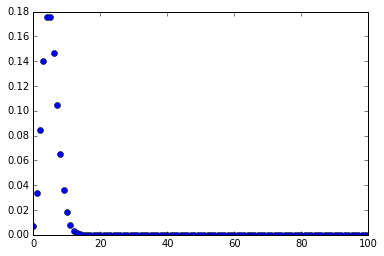
\includegraphics[height=7cm,keepaspectratio=true]{./pe/distPoisson0.png}
 % distPoisson0.png: 0x0 pixel, 300dpi, 0.00x0.00 cm, bb=
 \caption{Distribución de Poisson}
\end{figure}




\begin{figure}
 \centering
 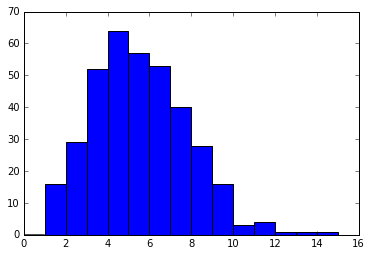
\includegraphics[height=7cm,keepaspectratio=true]{./pe/distPoisson1.png}
 % distPoisson1.png: 0x0 pixel, 300dpi, 0.00x0.00 cm, bb=
 \caption{Histograma de pacientes en sala de urgencias durante un año con media $\lam=5$}
 \label{fig:2.10.6}
\end{figure}



\subsection{Relación entre las Distribuciones Binomiales y de Poisson}

 Si en la función de probabilidad binomial, $N$ es muy grande pero $p \approx 0,$ esto modela un \emph{evento raro}.  En la práctica esto significa $N>>50, Np<<5.$

 En este caso, la distribución Binomial con parámetros $N,p$ se aproxima a una Poisson con parámetro $\lam = Np.$

\lstinputlisting[language=Python]{../code/distribuciones-especiales/relBinomPoisson.py}



 \begin{figure}
 \centering
 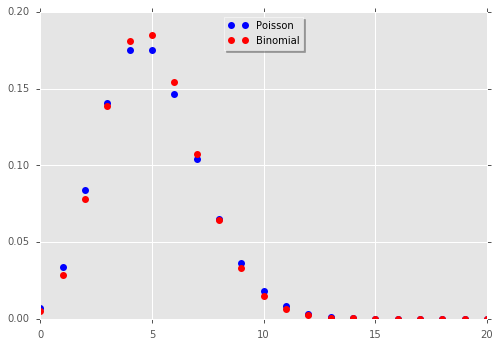
\includegraphics[height=7cm]{./pe/binVsPoi.png}
 % binVsPoi.png: 0x0 pixel, 300dpi, 0.00x0.00 cm, bb=
 \caption{Comparación entre distribuciones Binomial y Poisson para eventos raros.}
\end{figure}



\subsection{Aproximación normal a distribuciones discretas}
\subsubsection{Distribución Normal}

 Una de las distribuciones de probabilidad continua más importantes es la \emph{distribución normal}, también llamada \emph{distribución gaussiana,} que se define mediante la función de densidad
 \begin{align}
  \label{eq:2.10.4}
  f_{a,b}(x)=\dfrac{1}{\sqrt{2\pi}}e^{-\frac{1}{2}\frac{(x-a)^{2}}{b^{2}}}
 \end{align}
donde $a,b$ son parámetros específicos para cada v.a. $X.$

{Propiedades de la distribución normal}
 Si la v.a. $X$ tiene la función de densidad dada por \eqref{eq:2.10.4}, con parámetros $a,b$ entonces
 \begin{align}
  a = \mu_{X}\\
  b = \s_{X}
 \end{align}



 Si una variable aleatoria normal $X$ tiene función de densidad
  \begin{align}
  \label{eq:2.10.4a}
  f(x)=\dfrac{1}{\sqrt{2\pi}}e^{-\frac{1}{2}\frac{(x-\mu)^{2}}{\s^{2}}},
  \end{align}
  escribiremos $X\sim N(\mu, \s^{2}).$


{Variable aleatoria normalizada}
 \begin{align}
  \label{eq:2.10.5}
  Z = \dfrac{X-\mu}{\s}\\
  \mu_{Z}=0 \\
  \s_{Z}=1
 \end{align}


{Forma Estándar}
 \begin{align}
  \label{eq:2.10.6}
  f(z)=\dfrac{1}{\sqrt{2\pi}}e^{-\frac{1}{2}z^{2}}
 \end{align}


En este caso, diremos que $Z$ está \emph{normalmente distribuida.}


\lstinputlisting[language=Python]{../code/distribuciones-especiales/distribucionNormal.py}


 \begin{figure}
 \centering
 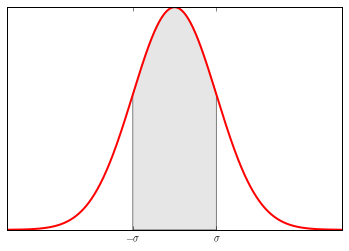
\includegraphics[height=5cm,keepaspectratio=true]{./pe/norm1.png}
 % norm1.png: 0x0 pixel, 300dpi, 0.00x0.00 cm, bb=
 \label{fig:2.10.2}
\end{figure}
\begin{verbatim}
 #(0.682689492137086, 7.579375928402476e-15)
\end{verbatim}


 \begin{figure}
 \centering
 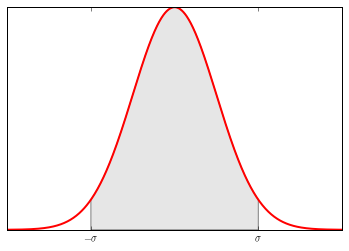
\includegraphics[height=5cm,keepaspectratio=true]{./pe/norm2.png}
 % norm1.png: 0x0 pixel, 300dpi, 0.00x0.00 cm, bb=
 \label{fig:2.10.3}
\end{figure}
\begin{verbatim}
 #(0.9544997361036417, 1.8403548653972355e-11)
\end{verbatim}


 \begin{figure}
 \centering
 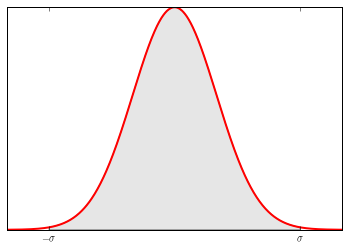
\includegraphics[height=5cm,keepaspectratio=true]{./pe/norm3.png}
 % norm1.png: 0x0 pixel, 300dpi, 0.00x0.00 cm, bb=
 \label{fig:2.10.4}
\end{figure}
\begin{verbatim}
 #(0.9973002039367399, 1.1072256503105314e-14)
\end{verbatim}


 \begin{figure}
 \centering
 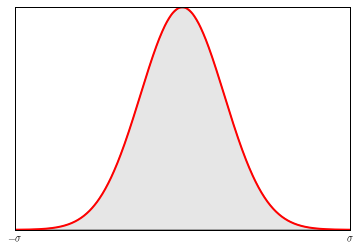
\includegraphics[height=5cm,keepaspectratio=true]{./pe/norm4.png}
 % norm1.png: 0x0 pixel, 300dpi, 0.00x0.00 cm, bb=
 \label{fig:2.10.5}
\end{figure}
\begin{verbatim}
 #(0.9999366575163339, 4.838904125482879e-12)
\end{verbatim}


\lstinputlisting[language=Python]{../code/distribuciones-especiales/normalCDF.py}
\begin{center}
 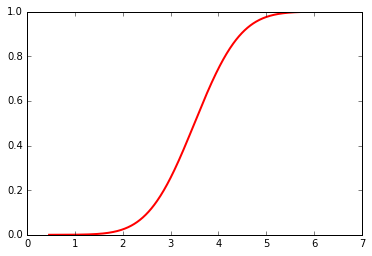
\includegraphics[height=5cm,keepaspectratio=true]{./pe/normCDF.png}
 % normCDF.png: 0x0 pixel, 300dpi, 0.00x0.00 cm, bb=
\end{center}



\subsubsection{Relación entre las distribuciones binomial y normal}

 Si $N\sim \infty, p,q>>0,$ y $X$ es un distribución binomial con parámetros $N,p$ entonces
 \begin{align}
  \dfrac{X-Np}{\sqrt{Npq}} \sim N(0,1).
 \end{align}



 \begin{ejemplo}
  \label{exmp:2.10.4}
  Consideremos el experimento de lanzar 16 veces una moneda. Repitamos 1,000,000 dicho experimento. Compruebe que dicho experimento se puede modelar por una variable aleatoria con distribución $N(\mu=8,\sigma^{2}=4)$
 \end{ejemplo}


\lstinputlisting[language=Python]{../code/distribuciones-especiales/relBinomNormal.py}
\begin{center}
 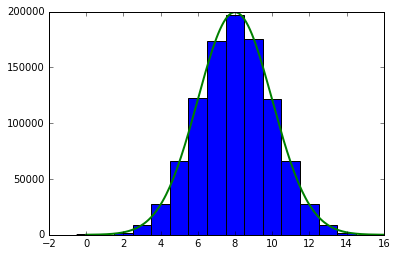
\includegraphics[height=5cm]{./pe/relBinNorm.png}
 % relBinNorm.png: 0x0 pixel, 300dpi, 0.00x0.00 cm, bb=
\end{center}


\subsubsection{Problemas Resueltos}
{Percentil}
 Diremos que $x=P_{q}$ es el percentil $q, \; 0\leq q \leq 100$ de la distribución $F(x)$ si $F(P_{q})=q\%.$  En el caso de que $q$ sea un valor realizable de $F(x),$ podemos \emph{``despejar''}
 \begin{align}
  P_{q}=F^{-1}\left( \dfrac{q}{100} \right).
 \end{align}
 A tal función se le llama \emph{distribución inversa.}


{Cuartiles}
 En la literatura se definen conceptos similares. Por ejemplo, el primer \emph{cuartil} corresponde al percentil $25;$ el segundo cuartil al percentil $50;$ y así sucesivamente.

{Combinaciones}
 \begin{ejemplo}
  \label{exmp:2.10.7}
  Encuentre
  \begin{enumerate}
   \item $5!$
   \item $\comb{8}{3}$
  \end{enumerate}
  utilizando \texttt{Python.}
 \end{ejemplo}


\lstinputlisting[language=Python]{../code/distribuciones-especiales/combinaciones.py}




{Distribución Binomial}
 \begin{ejemplo}
  \label{exmp:2.10.8}
  Supóngase que $15\%$ de la población es zurda. Encontrar la probabilidad de que en un grupo de 50 individuos haya:
  \begin{enumerate}
   \item cuando mucho 10 zurdos;
   \item por lo menos 5 zurdos;
   \item entre 3 y 6 zurdos;
   \item exactamente 5 zurdos.
  \end{enumerate}

 \end{ejemplo}


\lstinputlisting[language=Python]{../code/distribuciones-especiales/solvedBinom.py}



{Distribución Normal}
 \begin{ejemplo}
  \label{exmp:2.10.9}
  En un examen final de matemáticas, la media fue 72 y la desviación estándar fue 15. Determinar las puntuaciones estándar de los estudiantes que obtuvieron:
  \begin{enumerate}
   \item $60$;
   \item $93$;
   \item $72$.
  \end{enumerate}

 \end{ejemplo}



 \begin{ejemplo}
   \label{exmp:2.10.10}
   Con los datos del problema \ref{exmp:2.10.9}, encontrar las calificaciones que corresponden a las siguientes puntuaciones estándar:
  \begin{enumerate}
   \item $-1$;
   \item $1.6$.
  \end{enumerate}

 \end{ejemplo}



 \begin{ejemplo}
  \label{exmp:2.10.11}
  Supóngase que la cantidad de juegos en que participan los beisbolistas de la liga mayor durante su carrera se distribuye normalmente con media de $1500$ juegos y desviación estándar $350$ juegos. Emplear \texttt{Python} para responder las siguientes preguntas:
  \begin{enumerate}
   \item ¿Qué porcentaje participa en menos de 750 juegos?;
   \item ¿qué porcentaje participa en más de 2000 juegos?;
   \item encontrar el \emph{percentil} $90$ de la cantidad de juegos en los que participan en su carrera.
  \end{enumerate}

 \end{ejemplo}


\lstinputlisting[language=Python]{../code/distribuciones-especiales/solvedNorm.py}


{Eventos raros}
\begin{ejemplo}
\label{exmp:2.10.12}
  Si la probabilidad de que un individuo tenga una reacción adversa por la inyección de determinado suero es $0.001,$ determinar la probabilidad de que de 2000 individuos:
 \begin{enumerate}
  \item exactamente 3;
  \item más de 2
 \end{enumerate}
sufran una reacción adversa.
\end{ejemplo}


\lstinputlisting[language=Python]{../code/distribuciones-especiales/eventosRaros.py}


